\chapter{Prototype Methods and Nearest-Neighbors（原型方法与最近邻）}

% ============ §13.1 Introduction ============
\section{引言}

本章讨论一些\textbf{简单且本质上无模型}（model-free）的分类与模式识别方法。由于它们高度非结构化，通常不适合用来理解特征与类别结果之间关系的本质；但作为\textbf{黑箱预测引擎}（black box prediction engine），它们可以非常有效，常常是真实数据问题中表现最好的方法之一。

最近邻技术也可用于回归（第 2 章曾提及），在低维问题中表现合理。然而当特征维数较高时，最近邻回归的\textbf{偏差--方差权衡}不如分类情形有利，因此本章聚焦分类问题。

% ============ §13.2 Prototype Methods ============
\section{原型方法}

\begin{definition}[数据与原型]
训练数据为 $N$ 对 $(x_1,g_1),(x_2,g_2),\dots,(x_N,g_N)$，其中 $g_i$ 是取值于 $\{1,2,\dots,K\}$ 的类标签。\textbf{原型方法}（prototype methods）用特征空间中的一组点来表示训练数据，这些点称为\textbf{原型}（prototype）。原型通常\textbf{不是}训练样本本身（仅 $1$-最近邻分类除外，见后文）。每个原型带有一个类标签，查询点 $x$ 被分到\textbf{最近原型}所属的类。
\end{definition}

「最近」通常由特征空间中的\textbf{欧氏距离}定义，且每个特征先标准化为训练样本上的总体均值 $0$、方差 $1$。欧氏距离适用于定量特征；定性及其他类型特征值之间的距离度量在第 14 章讨论。

\begin{example}[原型：一个直观的例子]
设 $x=(x_1,x_2)$ 描述一只动物，$x_1$、$x_2$ 分别代表某两个特征（如体重与身高，已标准化到示意尺度），类标签 $g\in\{1,2\}$ 分别表示「猫」和「狗」。训练集共有 40 个样本（每类 20 个）。图 \ref{fig:13_prototype_example} 中，左下角蓝色小点是猫类样本、右上角绿色小点是狗类样本。

原型方法\textbf{不直接保存这 40 个样本}，而是先用某种算法（如 §13.2.1 的 K-means）为每个类挑出 $R=2$ 个「代表性」的点作为原型，例如：
\begin{align*}
\text{猫（类 1）}: &\quad m_1^{(1)} = (1.4,\,1.7),\quad m_2^{(1)} = (2.2,\,2.3),\\
\text{狗（类 2）}: &\quad m_1^{(2)} = (6.0,\,4.5),\quad m_2^{(2)} = (7.0,\,5.3).
\end{align*}
每个原型（图中方块）带一个类标签。于是整个训练集被\textbf{压缩}成 $K\times R = 4$ 个原型。

现在来了一个未知动物 $x=(3.4,\,3.2)$（图 \ref{fig:13_prototype_example} 中实心点）。计算它到 4 个原型的欧氏距离：
\begin{align*}
d(x,m_1^{(1)}) &= \norm{(2.0,1.5)} \approx 2.50, &
d(x,m_2^{(1)}) &= \norm{(1.2,0.9)} \approx 1.50,\\
d(x,m_1^{(2)}) &= \norm{(-2.6,-1.3)} \approx 2.91, &
d(x,m_2^{(2)}) &= \norm{(-3.6,-2.1)} \approx 4.17.
\end{align*}
最近的原型是 $m_2^{(1)}$（属于猫类），因此 $x$ 被分类为「猫」（图中红色箭头指向该原型）。

这个例子说明三个要点：
\begin{enumerate}[itemsep=1pt]
\item \textbf{原型是「代表点」，通常不是训练样本本身}——它们是特征空间中能概括一类数据分布的点；
\item \textbf{压缩表示}：分类时只需把 $x$ 与少数原型（这里是 4 个）比较距离，而无需与全部 40 个样本逐一比较，从而大幅降低存储与计算成本；
\item \textbf{1-最近邻是极端情形}：若 $R=N$（每个训练样本都保留为原型），就退化为 1-最近邻分类器——它\textbf{不压缩}，需要保存并比较全部数据。
\end{enumerate}
\end{example}

\begin{figure}[htbp]
\centering
\begin{tikzpicture}[>=stealth, font=\small, scale=1.0]
  % 坐标轴
  \draw[->] (0,0) -- (0,6.3) node[above]{$x_2$};
  \draw[->] (0,0) -- (8.6,0) node[right]{$x_1$};
  % 猫类样本（蓝色小点）
  \foreach \x/\y in {0.8/1.0,1.2/1.8,1.6/1.3,2.0/2.4,2.4/1.6,1.0/2.6,1.8/2.0,2.6/2.8}{
    \fill[blue!60!black] (\x,\y) circle (1.5pt);
  }
  % 狗类样本（绿色小点）
  \foreach \x/\y in {5.0/4.2,5.6/4.8,6.2/4.4,6.8/5.2,7.4/4.6,5.4/5.4,6.4/5.6,7.6/5.0}{
    \fill[green!50!black] (\x,\y) circle (1.5pt);
  }
  % 猫类原型（蓝色方块）
  \draw[blue, thick] (1.4,1.7) rectangle ++(0.34,0.34);
  \node[blue, below right] at (1.76,1.7) {$m_1^{(1)}$};
  \draw[blue, thick] (2.2,2.3) rectangle ++(0.34,0.34);
  \node[blue, above left] at (2.2,2.64) {$m_2^{(1)}$};
  % 狗类原型（绿色方块）
  \draw[green!50!black, thick] (6.0,4.5) rectangle ++(0.34,0.34);
  \node[green!50!black, right] at (6.36,4.5) {$m_1^{(2)}$};
  \draw[green!50!black, thick] (7.0,5.3) rectangle ++(0.34,0.34);
  \node[green!50!black, above] at (7.0,5.66) {$m_2^{(2)}$};
  % 查询点 x
  \fill[black] (3.4,3.2) circle (2.4pt);
  \node[black, above right] at (3.4,3.2) {$x$};
  % 到最近原型（m2^(1)，猫类）的连线
  \draw[red, thick, ->] (3.4,3.2) -- (2.5,2.6);
\end{tikzpicture}
\caption{原型方法示意：每类用两个原型（方块）代表大量训练样本（小点），查询点 $x$（实心点）被分到最近原型所属的类。}
\label{fig:13_prototype_example}
\end{figure}

\begin{remark}[有效性与挑战]
若原型定位得当，能很好地捕捉各类的分布，不规则类边界也可用足够多的原型放在正确位置来表示。主要挑战是：\textbf{用多少个原型、放在哪里}。不同方法按原型的选择数量与方式区分。
\end{remark}

% ============ §13.2.1 K-means Clustering ============
\subsection{K-means 聚类}

K-means 聚类是在\textbf{无标签}数据中寻找簇与簇中心的方法：先选定期望的簇中心个数 $R$，然后迭代移动中心以最小化\textbf{总簇内方差}。

\begin{remark}[符号约定]
K-means 中的「K」指簇中心个数。由于本书已用 $K$ 表示类别数，这里用 $R$ 表示簇的个数。
\end{remark}

给定一组初始中心，K-means 算法交替执行两步：

\begin{enumerate}[itemsep=1pt]
\item 对每个中心，识别出距离它比距其他任何中心都更近的训练点子集（即它的\textbf{簇}）；
\item 计算每个簇中各数据点的各特征均值，该均值向量成为该簇的新中心。
\end{enumerate}

这两步迭代直到收敛。通常初始中心是从训练数据中随机选取的 $R$ 个观测。K-means 的细节、允许不同变量类型与更一般距离度量的推广见第 14 章。

将 K-means 聚类用于\textbf{有标签数据的分类}，步骤如下：

\begin{enumerate}[itemsep=1pt]
\item 对每个类分别应用 K-means 聚类，每类使用 $R$ 个原型；
\item 给这 $K\times R$ 个原型分配类标签；
\item 将新特征 $x$ 分到最近原型所属的类。
\end{enumerate}

\paragraph{监督分类问题为什么用聚类（K-means）？}

关键是角色区分：这里的 K-means \textbf{不是最终分类器，而是「原型生成 / 数据压缩」的子程序}。监督信息（类标签）只决定两件事——每类用 $R$ 个原型、聚类完成后给每个原型贴类标签；而无监督的 K-means 只负责\textbf{在每一类内部}找出数据密集的「代表点」。上面的三个步骤中，第 1 步是\textbf{对每个类分别}单独聚类，第 2 步才用到类标签，第 3 步做分类。因此更准确的说法是：\textbf{用聚类作为「有监督分类」中生成原型的工具}，而不是「用无监督算法做分类」。§13.2.3 的高斯混合也是同样的角色，只是它是「软」的原型生成。

\begin{remark}[图 \ref{fig:13_1}（上）：K-means 的缺点]
三类两特征的模拟例子中取 $R=5$ 个原型/类。可以看到许多原型靠近类边界，导致边界附近的点可能被错分。这源于该方法一个明显的不足：\textbf{对每个类而言，其他类在定位该类的原型时没有发言权}。更好的方法（接下来讨论）用全部数据来定位所有原型。
\end{remark}

\paragraph{K-means 初始化原型时没有把类标签考虑进去吗？}

确实没有——这正是上一则注记所述不足的根源。对每类分别聚类时，原型的摆放只取决于本类数据分布，完全忽略类边界与类间重叠。后果如图 \ref{fig:13_1}（上）：许多原型落在靠近类边界的位置，边界附近的点易被错分；图 13.2 中 K-means 甚至把（错误的）蓝色原型放在西北角，且因只按距离分类而\textbf{无法忽略}它。

这正是作者紧接着引入 \textbf{LVQ}（§13.2.2）的原因：LVQ 用\textbf{全部数据（含类标签）}定位所有原型，靠「正确类吸引、错误类排斥」把原型\textbf{推离决策边界}（图 \ref{fig:13_1} 下），弥补 K-means 的缺陷。简言之：K-means 提供初始位置（但「盲」，不看标签），LVQ 用标签信息把原型重新摆放到位。

\begin{figure}[htbp]
\centering
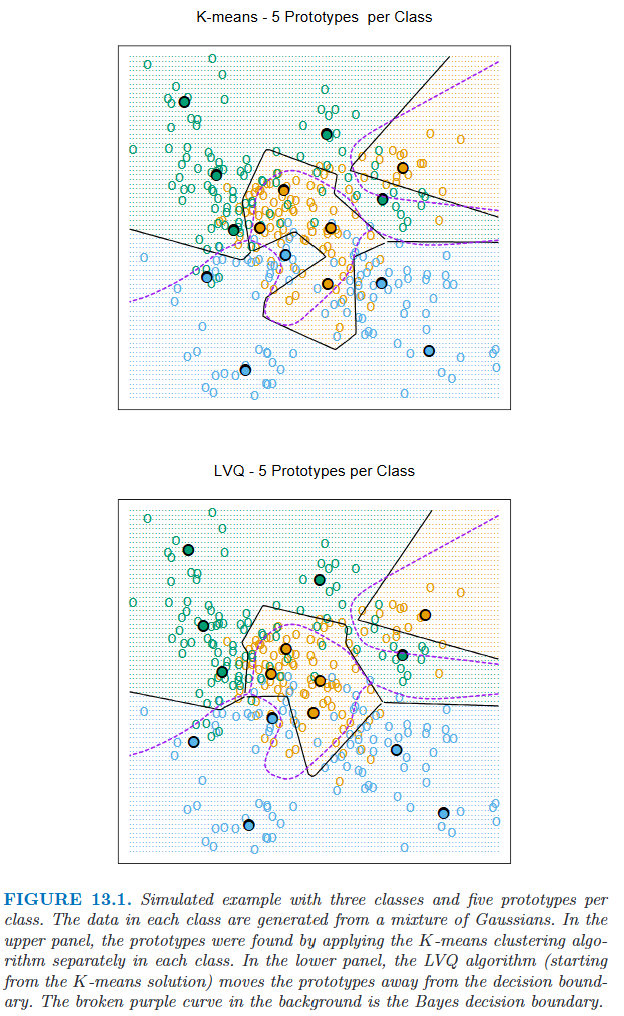
\includegraphics[width=0.95\textwidth]{Chapters/pic/ch_原型方法和最近邻/figure_13_1.png}
\caption{三类、每类五个原型的模拟例子（书图 13.1）。每类的数据由高斯混合生成。上方面板：对每类\textbf{分别}应用 K-means 聚类算法找到原型；下方面板：LVQ 算法（以 K-means 解为起点）把原型移离决策边界。背景中的紫色虚线是 Bayes 决策边界。}
\label{fig:13_1}
\end{figure}

% ============ §13.2.2 Learning Vector Quantization ============
\subsection{学习向量量化（LVQ）}

该技术源于 Kohonen (1989)，原型相对于决策边界\textbf{策略性地放置}。LVQ 是一种\textbf{在线算法}——观测被逐个处理。

其思想是：训练点\textbf{吸引}正确类的原型、\textbf{排斥}其他类的原型。迭代稳定后，原型应接近其所在类中的训练点。学习率 $\epsilon$ 随每次迭代递减至零，遵循随机近似学习率准则（见 §11.4）。

\begin{center}
\fbox{\parbox{0.92\textwidth}{%
\textbf{Algorithm 13.1（学习向量量化，LVQ）}\par\smallskip
\begin{enumerate}[itemsep=1pt]
\item 为每类选择 $R$ 个初始原型 $m_1^{(k)},m_2^{(k)},\dots,m_R^{(k)}$，$k=1,2,\dots,K$，例如从每类随机采样 $R$ 个训练点。
\item 随机（有放回）抽样一个训练点 $x_i$，记 $(j,k)$ 为距离 $x_i$ 最近的原型 $m_j^{(k)}$ 的索引：
\begin{itemize}[itemsep=1pt]
\item[(a)] 若 $g_i=k$（同属一类），将原型向训练点移动：
\begin{equation}
m_j^{(k)} \leftarrow m_j^{(k)} + \epsilon\bigl(x_i - m_j^{(k)}\bigr),
\end{equation}
其中 $\epsilon$ 为学习率；
\item[(b)] 若 $g_i\neq k$（属于不同类），将原型远离训练点移动：
\begin{equation}
m_j^{(k)} \leftarrow m_j^{(k)} - \epsilon\bigl(x_i - m_j^{(k)}\bigr).
\end{equation}
\end{itemize}
\item 重复第 2 步，学习率 $\epsilon$ 随每次迭代递减至零。
\end{enumerate}
}}
\end{center}

\begin{remark}[LVQ 的结果与不足]
图 \ref{fig:13_1}（下）展示了以 K-means 解为初值运行 LVQ 的结果：原型倾向于\textbf{远离决策边界}、远离竞争类的原型。上述过程实际称为 \textbf{LVQ1}；已有改进版本（LVQ2、LVQ3 等）有时可提升性能。LVQ 类方法的一个缺点是：它们由算法定义，而非优化某个固定准则，因此其性质难以理解。
\end{remark}

% ============ §13.2.3 Gaussian Mixtures ============
\subsection{高斯混合}

高斯混合模型也可视为一种原型方法，与 K-means 和 LVQ 精神类似（详见 §6.8、§8.5 与 §12.7）。每个簇由一个\textbf{高斯密度}描述：它既有\textbf{质心}（如同 K-means），又有\textbf{协方差矩阵}。若将分量高斯限制为\textbf{标量协方差矩阵}，与 K-means 的对比会更清晰（习题 13.1）。

交替 EM 算法的两步与 K-means 的两步非常相似：

\begin{itemize}[itemsep=1pt]
\item \textbf{E 步}：每个观测基于各对应高斯的似然，为每个簇分配一个\textbf{责任}（responsibility）或权重。靠近某簇中心的观测通常对该簇权重接近 1、对其他簇权重接近 0；位于两簇中间的观测则按比例分摊权重。
\item \textbf{M 步}：每个观测对每个簇的\textbf{加权均值}（和协方差）作出贡献。
\end{itemize}

因此高斯混合模型常被称为\textbf{软聚类}（soft clustering），而 K-means 是\textbf{硬聚类}。

\begin{remark}[软分类的实质]
当高斯混合模型用于表示每个类中的特征密度时，会为分类 $x$ 产生平滑的后验概率 $\hat{p}(x)=\{\hat{p}_1(x),\dots,\hat{p}_K(x)\}$（见式 (12.60)）。这常被解读为软分类，但实际分类规则仍是
\begin{equation}
\hat{G}(x) = \argmax_{k}\, \hat{p}_k(x).
\end{equation}

图 13.2 比较了 K-means 与高斯混合在第 2 章模拟混合问题上的结果：虽然决策边界大致相似，但混合模型的边界\textbf{更平滑}（尽管原型位置大致相同）。更重要的是，两种方法都在西北区域放置了一个（错误的）蓝色原型，但高斯混合分类器最终可以\textbf{忽略}这一区域，而 K-means 不能。高斯混合（公共协方差）测试误差约 $0.22$，K-means 约 $0.243$，Bayes 误差 $0.210$。
\end{remark}

% ============ §13.3 k-Nearest-Neighbor Classifiers ============
\section{k-最近邻分类器}

\begin{definition}[k-最近邻分类]
k-最近邻分类器是\textbf{基于记忆}（memory-based）的，无需拟合模型。给定查询点 $x_0$，找出距离它最近的 $k$ 个训练点 $x_{(r)},\ r=1,\dots,k$，然后在这 $k$ 个近邻中按\textbf{多数投票}分类；平局随机打破。
\end{definition}

为简单起见假设特征为实值，并使用特征空间中的欧氏距离：
\begin{equation}
d_{(i)} = \norm{x_{(i)} - x_0}. \label{eq:13_1}
\end{equation}

通常先把每个特征标准化为均值 $0$、方差 $1$（不同特征可能量纲不同）。第 14 章讨论定性/序数特征适用的距离度量及混合数据的组合方式；自适应选择的距离度量在本章后面讨论。

\begin{remark}[成功与适用场景]
尽管简单，k-最近邻在手写数字、卫星图像场景、EKG 模式等大量分类问题中非常成功。当每类有多个可能原型、且决策边界很不规则时，它往往表现优异。图 13.3 上方面板是 15-最近邻在三类模拟数据上的决策边界（相当平滑），下方面板是 1-最近邻（边界粗糙）。最近邻与原型方法联系紧密：在 1-最近邻分类中，\textbf{每个训练点都是一个原型}。
\end{remark}

\begin{remark}[偏差--方差与邻域大小]
图 13.4 展示了二类混合问题中训练、测试与十折交叉验证误差随邻域大小的变化（十折 CV 是十个数的平均，可估计标准误）。由于只用离查询点最近的训练点，1-最近邻估计的\textbf{偏差通常低但方差高}。简单最近邻的偏差/方差特性决定了给定问题的最优近邻数。
\end{remark}

\begin{theorem}[Cover--Hart 定理]
\textbf{渐近地}，1-最近邻分类器的错误率\textbf{不超过 Bayes 错误率的两倍}（Cover and Hart, 1967）。
\end{theorem}

\begin{remark}[证明思路（平方误差损失）]
假设查询点与某个训练点重合，则偏差为零（当特征空间维数固定、训练数据稠密填满空间时渐近成立）。于是 Bayes 规则的误差只是查询点目标（一个 Bernoulli 随机变量）的方差；而 1-最近邻规则的误差是 \textbf{两个} Bernoulli 随机变量（训练目标与查询目标）方差之和，即其两倍。
\end{remark}

\begin{remark}[误分类损失下的渐近分析]
在 $x$ 处令 $k^\ast$ 为主导类，$p_k(x)$ 为类 $k$ 的真实条件概率，则
\begin{align}
\text{Bayes 误差} &= 1 - p_{k^\ast}(x), \label{eq:13_2}\\
\text{1-最近邻误差} &= \sum_{k=1}^{K} p_k(x)\bigl(1-p_k(x)\bigr), \label{eq:13_3}\\
&\ge 1 - p_{k^\ast}(x). \label{eq:13_4}
\end{align}
渐近 1-最近邻错误率是一个\textbf{随机规则}的错误率：以概率 $p_k(x),\ k=1,\dots,K$ 随机选择分类与测试点。当 $K=2$ 时，1-最近邻错误率为
\[
2p_{k^\ast}(x)\bigl(1-p_{k^\ast}(x)\bigr) \le 2\bigl(1-p_{k^\ast}(x)\bigr),
\]
即 Bayes 错误率的两倍。更一般地可证明（习题 13.3）
\begin{equation}
\sum_{k=1}^{K} p_k(x)\bigl(1-p_k(x)\bigr) \le 2\bigl(1-p_{k^\ast}(x)\bigr) - \frac{K}{K-1}\bigl(1-p_{k^\ast}(x)\bigr)^2. \label{eq:13_5}
\end{equation}
Ripley (1996) 总结了大量此类结果。
\end{remark}

\begin{remark}[结果的应用与局限]
该结果可用于粗略估计某个问题可能达到的最佳性能：例如若 1-最近邻规则有 $10\%$ 错误率，则渐近 Bayes 错误率至少为 $5\%$。关键在于「渐近」部分——它假设最近邻规则的偏差为零；而\textbf{实际问题中偏差可能很大}。本章后面介绍的自适应最近邻规则正是为缓解这种偏差而设计的。
\end{remark}

% ============ §13.3.1 Example: A Comparative Study ============
\subsection{示例：比较研究}

在\textbf{两个模拟问题}上测试最近邻、K-means 与 LVQ 分类器。有 10 个独立特征 $X_j$，每个在 $[0,1]$ 上均匀分布；二类 0-1 目标变量定义为
\begin{equation}
\begin{aligned}
\text{问题 1（``简单''）} &: \quad Y = I\!\left(X_1 > \tfrac{1}{2}\right),\\
\text{问题 2（``困难''）} &: \quad Y = I\!\left(\sgn\!\left\{\prod_{j=1}^{3}\left(X_j - \tfrac{1}{2}\right)\right\} > 0\right).
\end{aligned} \label{eq:13_6}
\end{equation}

在问题 1 中，两类被超平面 $X_1=1/2$ 分开；问题 2 中，两类在前三个特征张成的超立方体内形成\textbf{棋盘图案}。两个问题的 Bayes 错误率均为零。训练集 100 个、测试集 1000 个观测。

图 13.5 展示了随调参参数变化的十次实现上最近邻、K-means 与 LVQ 错分误差的均值与标准误：

\begin{itemize}[itemsep=1pt]
\item K-means 与 LVQ 给出几乎相同的结果；在调参参数的最佳取值下，问题 1 中 K-means/LVQ 优于最近邻，问题 2 中二者表现相近。
\item 每个调参参数的最佳值\textbf{明显依赖具体情境}：例如问题 1 中 25-最近邻比 1-最近邻好约 $70\%$；而问题 2 中 1-最近邻最佳，比 25-最近邻好约 $18\%$。
\end{itemize}

这些结果强调了用\textbf{客观的、基于数据}的方法（如交叉验证，见图 13.4 与第 7 章）来估计调参参数最佳值的重要性。

% ============ §13.3.2 Example: k-NN and Image Scene Classification ============
\subsection{示例：k-最近邻与图像场景分类}

STATLOG 项目 (Michie et al., 1994) 用部分 \textbf{LANDSAT 卫星图像}作为分类基准（$82\times100$ 像素）。图 13.6 展示了澳大利亚某农区的四个热图波段（两个可见光、两个红外）。每个像素有来自 7 元素集合
\[
G = \{\text{红土，棉花，植被残茬，混合，灰土，湿灰土，很湿灰土}\}
\]
的类标签（由研究人员实地调查确定）。目标是根据四个光谱带的信息对像素的土地利用进行分类。

\textbf{5-最近邻}的预测地图按如下方式计算：对每个像素提取一个\textbf{8-邻域特征图}——像素本身及其 8 个直接邻居（图 13.7）。在四个光谱带分别这样做，得到每个像素 $(1+8)\times 4 = 36$ 个输入特征。然后在这个 36 维特征空间中进行 5-最近邻分类，测试错误率约 $\mathbf{9.5\%}$（图 13.8）。

\begin{remark}[STATLOG 结论]
在 STATLOG 项目使用的所有方法（包括 LVQ、CART、神经网络、线性判别分析等）中，k-最近邻在此任务上\textbf{表现最好}。由此推断，$\R^{36}$ 中的决策边界很可能相当不规则。
\end{remark}

% ============ §13.3.3 Invariant Metrics and Tangent Distance ============
\subsection{不变度量与切向距离}

在某些问题中，训练特征在某些自然变换下不变。最近邻分类器可以通过把这种不变性\textbf{并入距离度量}来加以利用。这里给出一个非常成功的例子（Simard et al., 1993）：\textbf{手写数字识别}，输入是 $16\times16=256$ 像素的灰度图像（示例见图 13.9）。

图 13.10 顶部展示了一个「3」的原始朝向（中间）及旋转 $\pm 7.5^\circ$、$\pm 15^\circ$ 的版本。手写中常出现这类旋转，人眼很容易看出小幅旋转后的「3」仍是「3」，因此希望最近邻分类器认为这些「3」彼此\textbf{接近}。然而，旋转「3」的 256 个灰度像素值与原始图像差异很大，两个对象在 $\R^{256}$ 的欧氏距离下可能\textbf{相距很远}。

\begin{definition}[不变流形与不变度量]
考虑由原始「3」及其旋转版本组成的像素值集合：这是 $\R^{256}$ 中的一条\textbf{一维曲线}，称为该图像在此变换下的\textbf{不变流形}（invariance manifold）。两幅图像之间的距离取为\textbf{第一个图像的任意变换版本与第二个图像的任意变换版本之间的最短欧氏距离}，称为\textbf{不变度量}（invariant metric）。
\end{definition}

\begin{remark}[不变度量的两个问题]
原则上可以用该不变度量进行 1-最近邻分类，但它有两个问题：其一，对真实图像很难计算；其二，它允许\textbf{过大的变换}导致性能下降——例如「6」旋转 $180^\circ$ 后会被认为接近「9」。因此需要把注意力限制在小旋转上。
\end{remark}

\textbf{切向距离}（tangent distance）同时解决这两个问题。如图 13.10 所示，可用原始图像处不变流形的\textbf{切线}来近似该流形。这条切线可通过小旋转图像估计方向向量来计算，也可用更精细的空间平滑方法（习题 13.4）。对于大旋转，切线图像不再像「3」，从而缓解了大变换带来的问题。

\begin{definition}[切向距离分类]
对每个训练图像计算其不变切线；对要分类的查询图像同样计算其不变切线，然后在训练集的所有切线中找\textbf{最近的一条切线}，该切线对应的类别即预测类别。图 13.11 中我们用的是\textbf{两条切线之间的最短距离}，而非两图像间欧氏距离或两曲线间最短距离。（图中两切线看似相交，只是因为在二维中示意实际的 256 维情形；在 $\R^{256}$ 中两条直线相交的概率实际上为零。）
\end{definition}

\begin{remark}[更简单的替代：hints]
实现这种不变性的更简单做法是把每个训练图像的若干旋转版本加入训练集，再用标准最近邻分类器。这一思想在 Abu-Mostafa (1995) 中称为 ``hints''，当不变空间较小时效果不错。但除旋转外，还有六种我们希望的变换不变性：平移（两个方向）、缩放（两个方向）、剪切、字符粗细。因此图 13.10/13.11 中的曲线与切线实际上是\textbf{7 维流形与超平面}。为每个训练图像加入所有这些变换版本不可行，而\textbf{切线流形优雅地捕获了这些不变性}。
\end{remark}

\begin{table}[htbp]
\centering
\caption{手写 ZIP 码问题的测试错误率（书表 13.1）。数据为美国邮政服务数据库：7291 个训练图像、2007 个测试数字。}
\label{tab:13_1}
\begin{tabular}{lc}
\toprule
方法 & 错误率 \\
\midrule
神经网络 & 0.049 \\
1-最近邻 / 欧氏距离 & 0.055 \\
1-最近邻 / 切向距离 & 0.026 \\
\bottomrule
\end{tabular}
\end{table}

\begin{remark}[结果与实践]
切向距离最近邻分类器效果惊人地好，测试错误率接近人眼水平（这是公认很难的测试集）。实际应用中最近邻对该在线分类任务而言\textbf{太慢}（见 §13.5），因此随后开发了神经网络分类器来模拟它。
\end{remark}

% ============ §13.4 Adaptive Nearest-Neighbor Methods ============
\section{自适应最近邻方法}

当最近邻分类在\textbf{高维}特征空间中进行时，一个点的最近邻可能\textbf{非常远}，从而引入偏差、降低规则性能。

\begin{remark}[维数灾难的量化]
考虑 $N$ 个数据点均匀分布在单位立方体 $[-\tfrac{1}{2},\tfrac{1}{2}]^p$ 中。设 $R$ 为原点处 1-最近邻域的半径，则
\begin{equation}
\operatorname{median}(R) = v_p^{-1/p}\left(1 - \left(\tfrac{1}{2}\right)^{1/N}\right)^{1/p}, \label{eq:13_7}
\end{equation}
其中 $v_pr^p$ 是 $p$ 维空间中半径 $r$ 的球体积。图 13.12 显示中位半径随样本量 $N$ 与维数 $p$ 的变化：中位半径\textbf{迅速逼近 0.5}——即到立方体边缘的距离。样本量需随维数指数级增长才能维持小的邻域。
\end{remark}

\begin{remark}[如何补救：自适应度量]
考虑图 13.13 的二类情形：两个特征，查询点处的最近邻域为圆形区域。最近邻分类隐含假设类概率在邻域内近似恒定、因而简单平均就能给出好的估计。但该例中类概率\textbf{只在水平方向变化}：若知道这一点，就应把邻域在垂直方向拉伸（如图中高矩形），这会在\textbf{保持方差不变的同时降低偏差}。

一般而言，这要求在最近邻分类中\textbf{自适应地选择度量}，使邻域沿类概率变化不大的方向拉伸。在高维特征空间中，类概率可能只在一个低维子空间变化，因此自适应度量可能带来显著优势。
\end{remark}

\begin{remark}[发展脉络]
Friedman (1994a) 提出一种方法：通过依次切除包含训练数据的盒子的边，自适应地找到矩形邻域。本节描述 Hastie and Tibshirani (1996a) 的\textbf{判别自适应最近邻}（discriminant adaptive nearest-neighbor, \textbf{DANN}）规则；更早的相关建议见 Short and Fukunaga (1981)、Myles and Hand (1990)。

在每个查询点处先形成一个约 50 个点的邻域，用其中的类分布决定如何\textbf{变形}邻域（即自适应度量），自适应度量再用于该查询点的最近邻规则。因此\textbf{每个查询点可能使用不同的度量}。
\end{remark}

在图 13.13 中，邻域显然应沿\textbf{连接类质心的直线的正交方向}拉伸。该方向也与线性判别边界重合，是类概率变化最小的方向。一般而言，最大变化方向并不正交于连接类质心的直线（见图 4.9，第 116 页）。假设局部判别模型成立，则局部\textbf{类内}与\textbf{类间}协方差矩阵所含信息足以确定邻域的最优形状。

\begin{definition}[DANN 度量]
查询点 $x_0$ 处的判别自适应最近邻（DANN）度量定义为
\begin{equation}
D(x,x_0) = (x - x_0)^T\,\Sigma\,(x - x_0), \label{eq:13_8}
\end{equation}
其中
\begin{equation}
\Sigma = W^{-1/2}\left[W^{-1/2} B\, W^{-1/2} + \epsilon I\right]W^{-1/2}
      = W^{-1/2}\left[B^\ast + \epsilon I\right]W^{-1/2}. \label{eq:13_9}
\end{equation}
这里 $W = \sum_{k=1}^{K}\pi_k W_k$ 是\textbf{合并的类内协方差矩阵}，$B = \sum_{k=1}^{K}\pi_k(\bar{x}_k - \bar{x})(\bar{x}_k - \bar{x})^T$ 是\textbf{类间协方差矩阵}，其中 $W$ 与 $B$ 只用 $x_0$ 周围约 50 个最近邻计算。算出度量后，再把它用于 $x_0$ 处的最近邻规则。
\end{definition}

\begin{remark}[Σ 的操作理解]
这个复杂的公式操作上其实很简单：
\begin{enumerate}[itemsep=1pt]
\item 先用 $W$ 对数据\textbf{球化}（sphering）；
\item 再在 $B^\ast$（球化后数据的类间矩阵）的\textbf{零特征值方向}上拉伸邻域。
\end{enumerate}
这很合理：这些方向上局部观测到的各类均值没有差异。参数 $\epsilon$ 把邻域从无限条带\textbf{圆整为椭球}，避免使用离查询点太远的点；$\epsilon=1$ 通常效果不错。

图 13.14 展示了同心圆（一类包围另一类）问题中 DANN 找到的邻域：当邻域内两类同时存在时，邻域沿与决策边界正交的方向拉伸；在只有一类的\textbf{纯净区域}，邻域保持圆形——此时类间矩阵 $B=0$，式 (13.8) 中的 $\Sigma$ 为单位阵。
\end{remark}

% ============ §13.4.1 Example ============
\subsection{示例}

这里生成十维二类数据，与图 13.14 的二维例子类似：类 1 的所有十个预测变量为独立标准正态，且\textbf{条件于平方半径} $22.4 < \norm{x}^2 < 40$；类 2 的预测变量为无限制的独立标准正态。每类 250 个观测。因此类 1 在完整十维空间中几乎完全包围类 2。

\begin{remark}[本例特点]
本例没有最近邻子集选择规则可以剔除的\textbf{纯噪声变量}：在特征空间的任意给定点，判别只沿\textbf{一个方向}发生，但该方向随空间位置变化，\textbf{所有变量在空间的某处都是重要的}。

图 13.15 展示十次实现上测试错误率的箱线图，比较标准 5-最近邻、LVQ 与判别自适应 5-最近邻。LVQ 每类使用 50 个原型（$250/5=50$，使其与 5-最近邻可比）。自适应度量相对 LVQ 或标准最近邻\textbf{显著降低了错误率}。
\end{remark}

% ============ §13.4.2 Global Dimension Reduction for Nearest-Neighbors ============
\subsection{最近邻的全局降维}

判别自适应最近邻方法进行的是\textbf{局部}降维——即在每个查询点分别降维。许多问题还可以受益于\textbf{全局降维}：在原始特征空间某个最优选择的\textbf{子空间}中应用最近邻规则。

例如，假设两类在四维特征空间中形成两个\textbf{嵌套球}，另有六个与类无关的噪声特征。那么我们希望对数据\textbf{发现重要的四维子空间}，并在该降维子空间中进行最近邻分类。

Hastie and Tibshirani (1996a) 为此讨论了判别自适应最近邻方法的一种变体：在每个训练点 $x_i$ 处计算\textbf{类间质心平方和矩阵} $B_i$，然后对所有训练点取平均：
\begin{equation}
\bar{B} = \frac{1}{N}\sum_{i=1}^{N} B_i. \label{eq:13_10}
\end{equation}

\begin{definition}[全局最优子空间]
设 $e_1,e_2,\dots,e_p$ 为矩阵 $\bar{B}$ 的特征向量，按特征值 $\theta_k$ 从大到小排列。这些特征向量\textbf{张成全局子空间约简的最优子空间}。其推导基于如下事实：$\bar{B}$ 的最佳秩 $L$ 逼近
\begin{equation}
\bar{B}_{[L]} = \sum_{\ell=1}^{L} \theta_\ell\, e_\ell e_\ell^T
\end{equation}
求解如下的最小二乘问题：
\begin{equation}
\min_{\operatorname{rank}(M)=L}\ \sum_{i=1}^{N} \tr\left[(B_i - M)^2\right]. \label{eq:13_11}
\end{equation}
\end{definition}

\begin{remark}[理解与联系]
每个 $B_i$ 含有 (a) 局部判别子空间的信息，以及 (b) 该子空间中判别强度的信息，因此式 (13.11) 可看作对一系列 $N$ 个子空间按加权最小二乘寻找最优 $L$ 维逼近子空间（习题 13.5）。

在四维球例子中，$\bar{B}$ 的四个特征值 $\theta_\ell$ 很大（其特征向量几乎张成感兴趣的子空间），其余六个接近零。操作上，把数据投影到前四维子空间后做最近邻分类即可。在 §13.3.2 的卫星图像分类例子中，图 13.8 标注为 DANN 的技术正是使用了全局降维子空间中的 5-最近邻。

该技术与 Duan and Li (1991) 的\textbf{切片逆回归}（sliced inverse regression）也有联系：后者在回归设定中使用类似思想，但做\textbf{全局}而非局部计算，并假设特征分布具有球对称性来估计感兴趣的子空间。
\end{remark}

% ============ §13.5 Computational Considerations ============
\section{计算考虑}

最近邻规则的一个普遍缺点是\textbf{计算负载}——既包括找近邻，也包括存储整个训练集。有 $N$ 个观测、$p$ 个预测变量时，每个查询点找近邻需要 $Np$ 次运算。已有更快的找最近邻算法（Friedman et al., 1975, 1977）可降低部分负载。Hastie and Simard (1998) 通过在不变度量下开发 K-means 聚类的类似物，减少了\textbf{切向距离}的计算量。

\textbf{降低存储需求}更困难，已有各种\textbf{编辑}（editing）与\textbf{压缩}（condensing）程序被提出：

\begin{itemize}[itemsep=1pt]
\item \textbf{思想}：隔离出足以进行最近邻预测的训练集子集，丢掉其余训练数据。直觉上应保留\textbf{靠近决策边界且位于边界正确一侧}的训练点，而可丢弃远离边界的点。
\item \textbf{多编辑算法}（Devijver and Kittler, 1982）：把数据循环地分成训练集与测试集，在训练集上计算最近邻规则，删除被错分的测试点——目的是保留同质的观测簇。
\item \textbf{压缩程序}（Hart, 1968）：更进一步，只保留簇的重要\textbf{外部点}。从随机选出的单个观测作为训练集开始，每个附加数据项逐个处理，仅当它被当前训练集上的最近邻规则\textbf{错分}时才加入训练集。
\end{itemize}

这些程序综述见 Dasarathy (1991) 与 Ripley (1996)，也可应用于最近邻以外的其他学习程序。本章书目注记（Bibliographic Notes）与习题从略。

% ============ 本章总结 ============
\section{本章总结}

\begin{figure}[htbp]
\centering
\begin{tikzpicture}[>=stealth, font=\small, scale=0.88, transform shape,
  box/.style={draw, rounded corners, align=center, inner sep=5pt, text width=3.2cm},
  note/.style={align=center, text width=2.7cm, font=\scriptsize, gray!60!black}]
  % 顶层
  \node[box, fill=blue!12] (top) at (0,0) {\textbf{无模型分类方法}\\不显式建模特征--类别关系};
  % 两大分支
  \node[box, fill=green!12] (proto) at (-4.4,-2.2) {\textbf{原型方法}\\$R$ 个原型，压缩 $N\to R$};
  \node[box, fill=orange!12] (nn) at (4.4,-2.2) {\textbf{最近邻方法}\\训练点即原型，记忆式、不压缩};
  \draw[->] (top.south) .. controls (-3.2,-1.0) .. (proto.north);
  \draw[->] (top.south) .. controls (3.2,-1.0) .. (nn.north);
  % 原型三兄弟
  \node[box] (km) at (-6.6,-4.5) {\textbf{K-means}\\类内硬聚类};
  \node[box] (lvq) at (-4.4,-8.0) {\textbf{LVQ}\\标签吸引 / 排斥};
  \node[box] (gm) at (-2.2,-4.5) {\textbf{高斯混合}\\软聚类};
  \draw[->] (proto.south) -- (km.north);
  \draw[->] (proto.south) -- (lvq.north);
  \draw[->] (proto.south) -- (gm.north);
  \node[note] at (-6.6,-6.2) {未用类标签，\\原型易靠近类边界};
  \node[note] at (-4.4,-9.5) {用全部数据，\\原型远离决策边界};
  \node[note] at (-2.2,-6.2) {平滑后验 $\hat p(x)$\\$\argmax_k \hat p_k(x)$};
  % 最近邻链
  \node[box] (knn) at (4.4,-4.5) {\textbf{$k$-NN}\\多数投票};
  \draw[->] (nn.south) -- (knn.north);
  \node[note] at (8.0,-4.5) {Cover--Hart：渐近\\$1$-NN 误差 $\le 2\times$Bayes};
  \node[box] (td) at (4.4,-6.9) {\textbf{不变度量 / 切向距离}\\以切线近似不变流形};
  \draw[->] (knn.south) -- (td.north);
  \node[note] at (8.0,-6.9) {旋转、平移、缩放、\\剪切、粗细等 7 维};
  \node[box] (dann) at (4.4,-11.0) {\textbf{自适应最近邻（DANN）}\\局部度量 + 全局降维};
  \draw[->] (td.south) -- (dann.north);
  \node[note] at (8.0,-11.0) {局部类内 $W$ / 类间 $B$\\$\bar B$ 特征子空间};
\end{tikzpicture}
\caption{本章方法总览：原型方法（压缩）与最近邻方法（记忆式）两大分支及其变体。}
\label{fig:13_summary}
\end{figure}

本章介绍了一族\textbf{无模型}（model-free）的分类方法：它们不显式估计特征与类别之间的关系，而是把分类建立在\textbf{距离 / 邻近性}之上。方法可按是否\textbf{压缩数据}分为两大范式（图 \ref{fig:13_summary}）：

\begin{description}[itemsep=2pt,leftmargin=1em]
\item[\textbf{原型方法}——压缩 $N\to R$：] 用每类 $R$ 个原型点代表训练数据，查询点分给最近原型。三种原型生成方式：
\begin{itemize}[itemsep=1pt]
\item \textbf{K-means}：对每类\textbf{分别}做硬聚类取 $R$ 个中心。定位原型时\textbf{未利用类标签}（「盲」），原型易靠近类边界（图 \ref{fig:13_1} 上）。
\item \textbf{LVQ}：用\textbf{全部数据含标签}在线更新——正确类吸引、错误类排斥，把原型\textbf{推离决策边界}（图 \ref{fig:13_1} 下）。
\item \textbf{高斯混合}：软聚类（EM 分配责任权重），得到平滑后验 $\hat p(x)$，分类取 $\argmax_k \hat p_k(x)$。
\end{itemize}

\item[\textbf{最近邻方法}——记忆式、不压缩：] 每个训练点即原型（$R=N$）。
\begin{itemize}[itemsep=1pt]
\item \textbf{$k$-NN}：多数投票；\textbf{Cover--Hart 定理}保证渐近 $1$-NN 误差不超过 $2\times$ Bayes 率。
\item \textbf{不变度量 / 切向距离}：把旋转、平移、缩放、剪切、粗细等不变性并入度量（以切线近似不变流形），把手写数字 $1$-NN 错误率从 $5.5\%$ 降到 $2.6\%$（表 \ref{tab:13_1}）。
\item \textbf{自适应最近邻（DANN）}：高维下最近邻退化（邻域半径迅速逼近立方体边缘，式 \ref{eq:13_7}）；DANN 用局部类内 $W$ 与类间 $B$ 协方差自适应度量（式 \ref{eq:13_8}--\ref{eq:13_9}），全局降维用 $\bar B$ 的特征子空间（式 \ref{eq:13_10}--\ref{eq:13_11}）。
\end{itemize}
\end{description}

贯穿全章的\textbf{核心权衡}：
\begin{itemize}[itemsep=1pt]
\item \textbf{偏差--方差}：$k$ 越小偏差越低、方差越高；最优 $k$ 依赖具体问题，需交叉验证选择（§13.3.1）。
\item \textbf{压缩 vs 记忆}：原型数 $R$ 决定压缩比与保真度；$R$ 越大保留信息越多，但存储与计算成本越高。
\item \textbf{计算}：每查询点需 $Np$ 次比较；可用编辑/压缩程序剪枝训练集（§13.5）。
\end{itemize}

一句话概括：方法越结构化越利于\textbf{解释}，越无模型越利于\textbf{黑箱预测}——当决策边界极不规则、每类原型众多时，最近邻及其变体往往是真实数据上表现最好的选择（如 STATLOG 36 维场景，§13.3.2）。
